\chapter{System Description}
In this project a quadcopter is provided with motors, motor controllers, propellers and a battery. The system in its initial state is seen on \autoref{fig:systemBase}. Apart from the quadcopter and the attached hardware, a tracking system called Vicon is also provided. This is used to track the quadcopter and provide it with sensor inputs.

\begin{figure}[H]
  \centering
  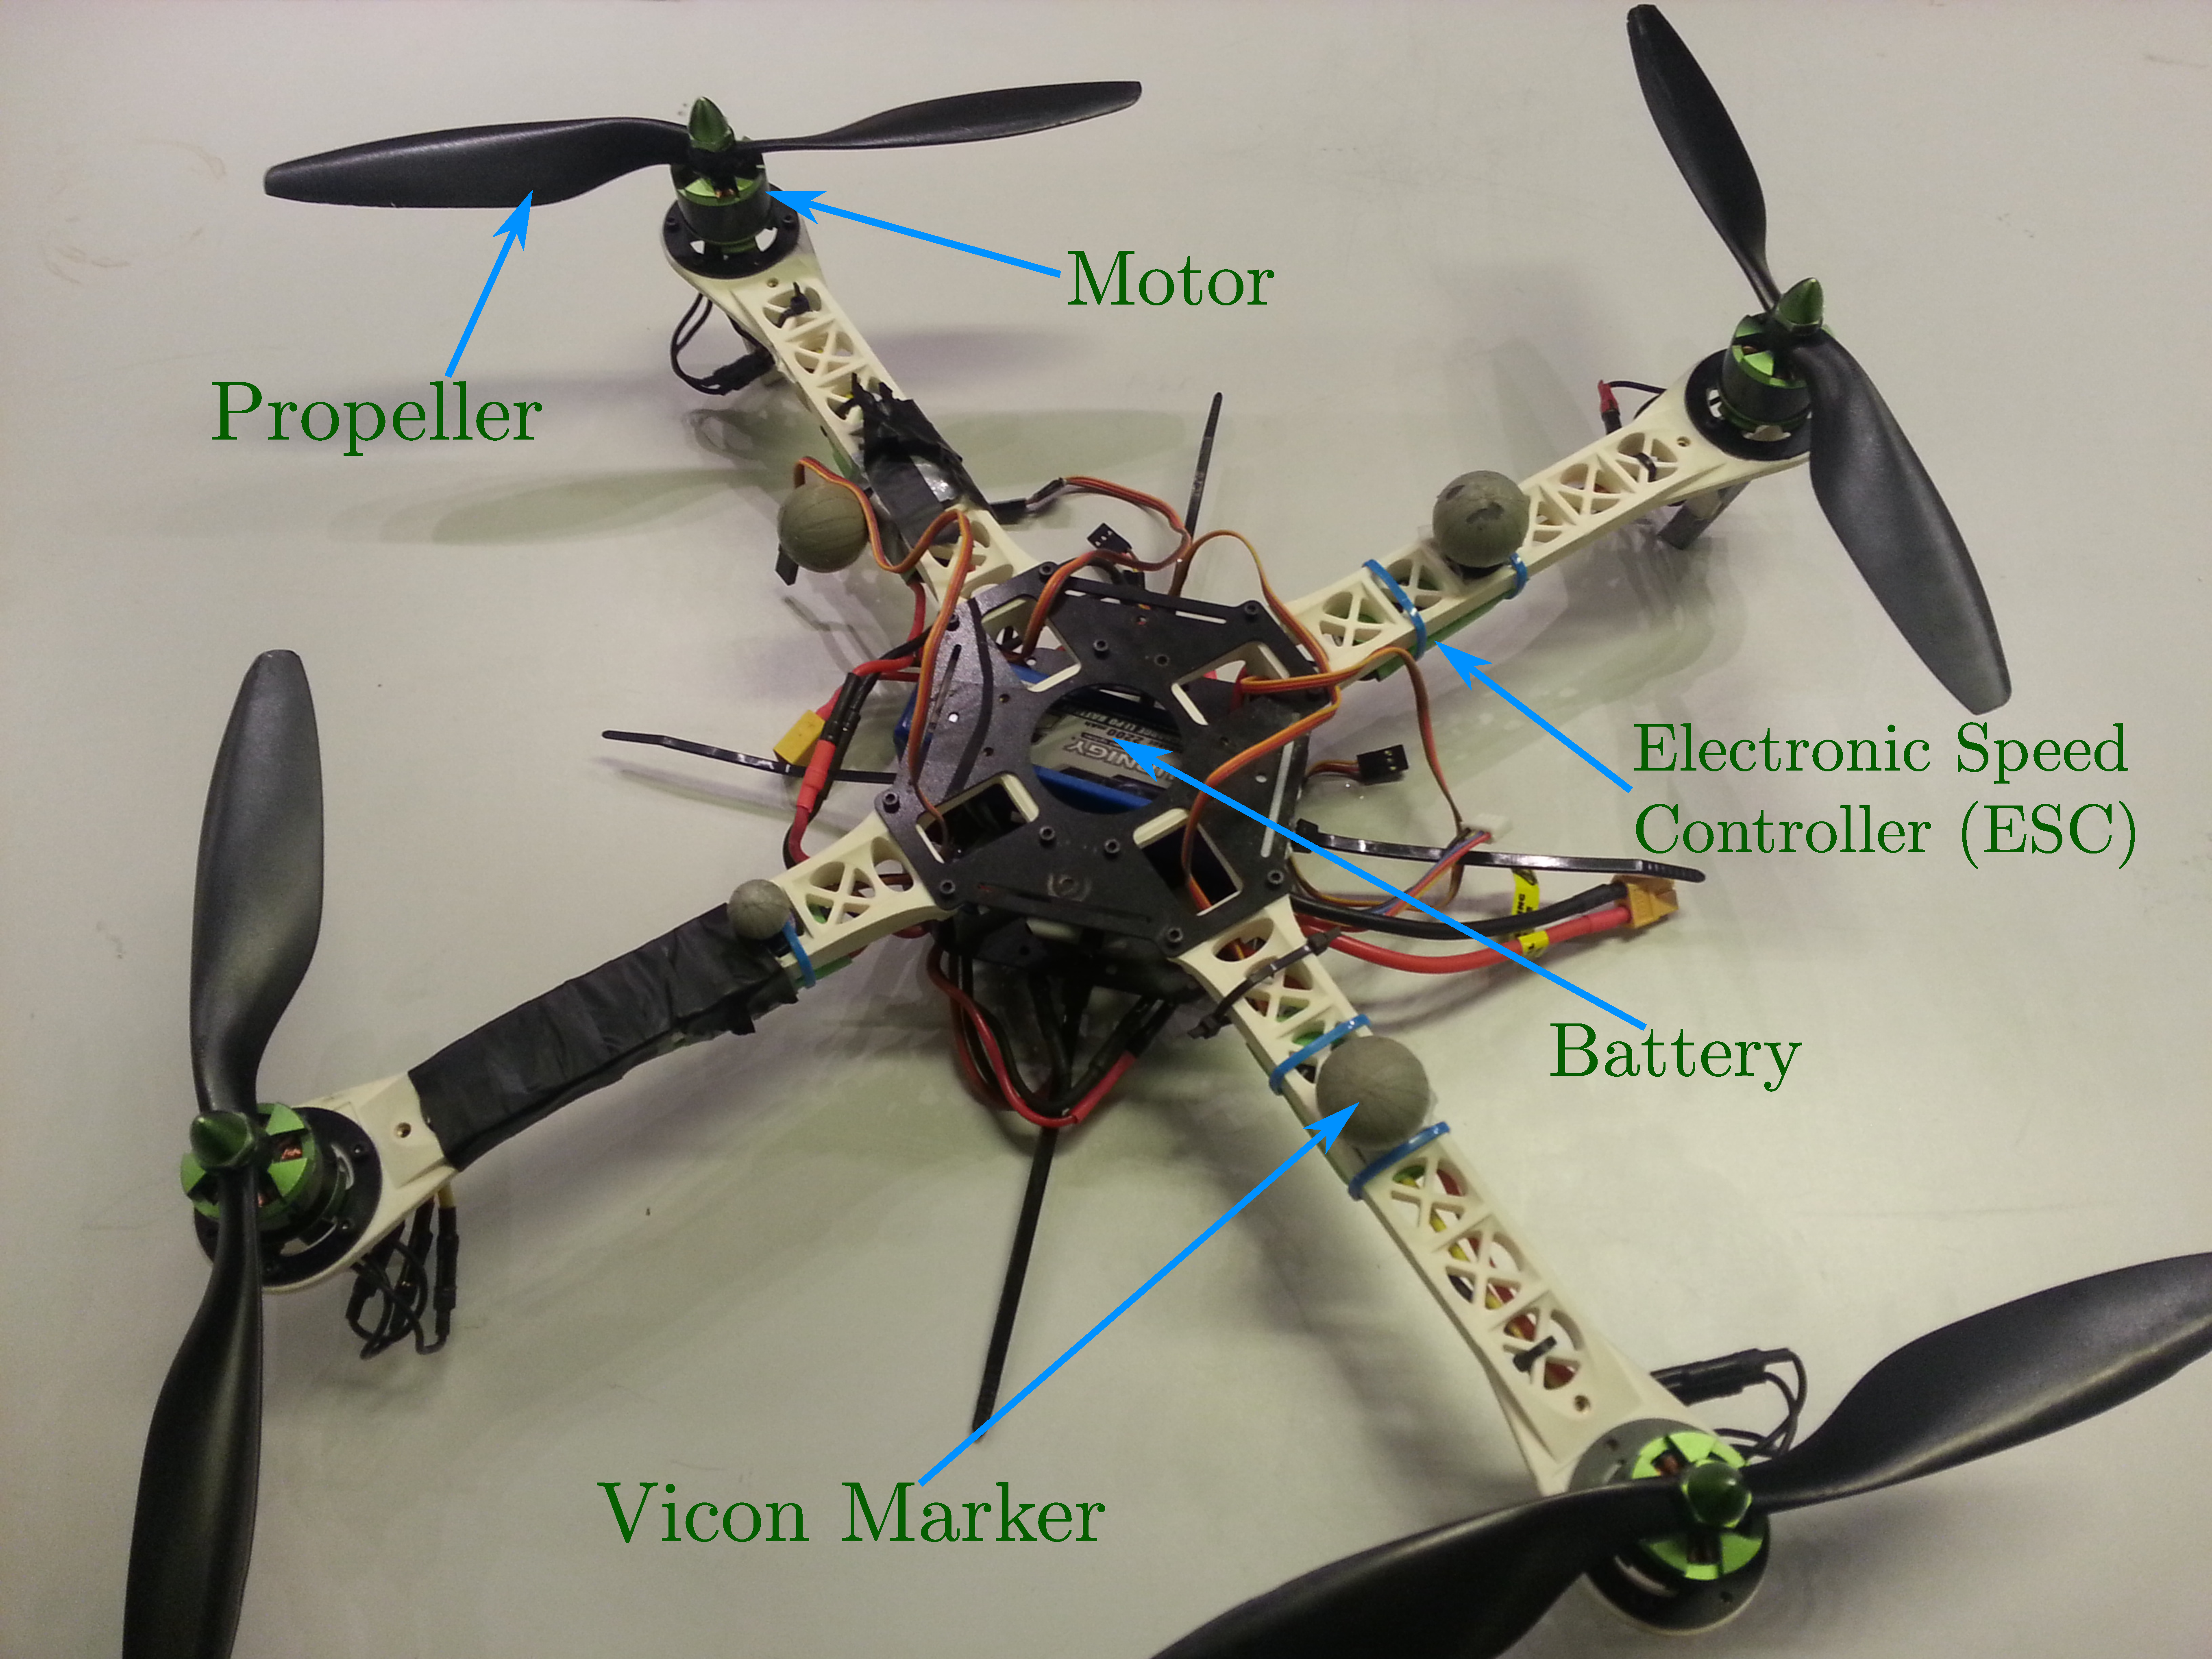
\includegraphics[width=.6\linewidth]{figures/quadcopterBaseLabels}
  \caption{The quadcopter with attached hardware as given.}
  \label{fig:systemBase}
\end{figure}

In this chapter all the given hardware is presented after which the overall structure of the prototype is described.